% ==========================================
% LatexRefinement Step Output: step4-04-14-25-tuesday-all-offset-final.tex
% Model: gemini-3.5-flash
% Temperature: 0.33
% TopP: 0.95
% TopK: 40
% MaxOutputTokens: 65535
% ThinkingBudget: 32765
% ThinkingLevel: HIGH
% Prompt Tokens: 40'347
% Candidates Tokens: 20'581 (inkl. Thinking Tokens)
% Cached Tokens: 0
% Processed on: 2026-07-15 20:39:54
% ==========================================

% ==========================================
% LatexRefinement Step Output: step3-04-14-25-tuesday-all-offset-speech_refined.tex
% Model: gemini-3.5-flash
% Temperature: 0.36
% TopP: 0.95
% TopK: 40
% MaxOutputTokens: 65535
% ThinkingBudget: 32765
% ThinkingLevel: HIGH
% Processed on: 2026-07-15 20:24:23
% ==========================================

\lecturechapter[8]{Dienstag}{14. Apr}{14. April 2026}{Das Auswahlaxiom, Ordinalzahlen und Äquivalenzen}
% Old chapter title: Auswahlaxiom und Ordinalzahlen

\begin{nice-box}[Vorlesungsübersicht \& Kontext]
In dieser Vorlesung vertiefen wir unser Verständnis des Auswahlaxioms und seiner weitreichenden Konsequenzen in der modernen Mathematik. Wir führen die Theorie der Ordinalzahlen ein und untersuchen fundamentale Beweisprinzipien wie die transfinite Induktion und Rekursion.

Die Hauptthemen dieser Vorlesung sind:
\begin{itemize}
    \item \textbf{Das Auswahlaxiom (AC):} Formale Definition, Auswahlfunktionen und die Äquivalenz zum kartesischen Produkt.
    \item \textbf{Ordinalzahlen:} Transitivität, Wohlordnung, Nachfolger- und Limes-Ordinalzahlen sowie geometrische Veranschaulichung.
    \item \textbf{Transfinite Methoden:} Transfinite Induktion und Rekursion mit Anwendungen wie dem Basisexistenzsatz für Vektorräume.
    \item \textbf{Äquivalenzen zum Auswahlaxiom:} Wir besprechen das Kuratowski-Zorn-Lemma (KZL), das Teichmüller-Prinzip (TP) sowie den vollständigen Beweis ihres Äquivalenzsatzes.
\end{itemize}
\end{nice-box}

\section{Das Auswahlaxiom}
\subsection{Einführung und formale Definition}

\begin{spoken-clean}[00:00:00 - 00:01:05]
So, hallo zusammen und herzlich willkommen zu dieser zweiten Hälfte des Semesters. Ich hoffe, Sie hatten alle schöne, erholsame\dots Osterferien. Das letzte Mal war ja Fabian Ziltener hier und hat mich vertreten --- hoffentlich --- und hat Ihnen vom Auswahlaxiom erzählt. Da werden wir jetzt fortfahren.

Ich hoffe natürlich, Sie haben über die Ferien jetzt nicht schon alles darüber vergessen. Aber da ich das letzte Mal nicht dabei war, wäre es vielleicht gar nicht schlecht, nochmals kurz durchzugehen, wo wir stehen. Sie haben das Auswahlaxiom gesehen --- das \emph{Axiom of Choice}. Wissen Sie noch, was das besagt? Gut, es gibt viele Möglichkeiten, das zu formulieren. Ja?
\end{spoken-clean}

\begin{student-interaction}[Studentenantwort]
Wir haben eine Familie von Mengen, also eine Menge von Mengen, und es ist immer möglich, dass wir aus jeder von dieser Menge ein Element auswählen gleichzeitig.
\end{student-interaction}

\begin{spoken-clean}[00:01:05 - 00:02:40]
Genau, absolut richtig! Wir haben eine Familie von Mengen --- also eine Menge von Mengen ---, und es ist immer möglich, dass wir aus jeder dieser Mengen gleichzeitig ein Element auswählen. Und diese Familie von Mengen soll natürlich nicht die leere Menge enthalten, weil es dann offensichtlich nicht geht --- aus der leeren Menge können wir schließlich nie ein Element auswählen.

Formal ausgedrückt sagt uns das Auswahlaxiom: Für alle $\mathcal{F}$ gilt, wenn die leere Menge nicht in der Familie $\mathcal{F}$ enthalten ist, dann existiert eine Funktion $f$. Und diese Funktion $f$ ist jetzt eben eine Auswahlfunktion; sie soll jedem Element dieser Familie von Mengen ein Element aus dieser Menge zuordnen. Das heißt, wir wollen eine Funktion, die von $\mathcal{F}$ --- also von dieser Familie --- in die Vereinigung $\bigcup \mathcal{F}$ geht. Für jede Menge $X \in \mathcal{F}$ erhalten wir also ein Element, das in dieser Menge $X$ enthalten ist. Wir wollen nun aber, dass für alle $X \in \mathcal{F}$ gilt: $f(X) \in X$.
\end{spoken-clean}

\begin{math-stroke}[Das Auswahlaxiom]
Das \newterm{Auswahlaxiom} ($\text{AC}$ -- Axiom of Choice) lässt sich formal als folgende Aussage in der Sprache der Mengenlehre formulieren:
\begin{equation}
\label{eq:axiom-of-choice}
\text{AC} \equiv \forall \mathcal{F} \left( \emptyset \notin \mathcal{F} \rightarrow \exists f \left( f \in {}^{\displaystyle\mathcal{F}}\!\bigcup \mathcal{F} \;\wedge\; \forall X \in \mathcal{F} \, \bigl( f(X) \in X \bigr) \right) \right)
\end{equation}
Hierbei bezeichnet $\mathcal{F}$ ein Mengensystem (eine Kollektion von Mengen) und die Vereinigung aller Elemente von $\mathcal{F}$ ist definiert durch:
\[
\bigcup \mathcal{F} := \bigcup_{X \in \mathcal{F}} X = \{ x \mid \exists X \in \mathcal{F} \text{ mit } x \in X \}
\]
Eine solche Funktion $f$ heißt \newterm{Auswahlfunktion} (Choice function).

\inlinemetanote{[Anmerkung: Die Notation ${}^{\mathcal{F}}\!\bigcup \mathcal{F}$ bezeichnet die Menge aller Abbildungen von der Familie $\mathcal{F}$ in ihre Vereinigungsmenge $\bigcup \mathcal{F}$. Das Auswahlaxiom garantiert die Existenz einer solchen Abbildung $f$, die aus jeder nicht-leeren Menge $X \in \mathcal{F}$ ein repräsentatives Element auswählt, sodass $f(X) \in X$ gilt.]}
\end{math-stroke}

\subsection{Äquivalente Formulierung des Auswahlaxioms}
\begin{spoken-clean}[00:02:40 - 00:03:50]
Das ist eine etwas umständliche Art und Weise aufzuschreiben, was wir eigentlich wollen: dass wir aus jeder Menge einer Familie von Mengen ein Element auswählen können. In Worten ausgedrückt: Jede Familie von nicht-leeren Mengen besitzt eine Auswahlfunktion. Und Sie haben gesehen, das ist auch wieder äquivalent zu der Aussage, dass das kartesische Produkt nicht-leerer Mengen nicht leer ist.
\end{spoken-clean}

\begin{math-stroke}[Äquivalente Formulierung des Auswahlaxioms]
\begin{proposition}[Äquivalenz zum kartesischen Produkt]\label[proposition]{prop:ac-equivalenz}
Das Auswahlaxiom ($\text{AC}$) ist äquivalent zu der folgenden Aussage:
\[
\text{Das kartesische Produkt nicht-leerer Mengen ist nicht leer.}
\]
\end{proposition}
\end{math-stroke}

\begin{spoken-clean}[00:03:50 - 00:05:29]
So ausgedrückt erscheint es eigentlich sehr sinnvoll, das als Axiom zu haben. Es wäre schließlich sehr, sehr schlecht, wenn wir in der Mathematik arbeiten würden und nicht wüssten, ob ein Produkt von nicht-leeren Mengen leer sein könnte. Aber das folgt eben nicht aus den Zermelo-Fraenkel-Axiomen; man muss es wirklich als zusätzliches Axiom annehmen.

Dennoch ist es von der Formulierung her vielleicht etwas, das man lieber beweisen würde. Als Axiom wirkt es doch ein bisschen umständlicher, als beispielsweise nur zu sagen: \qt{Die leere Menge existiert.} Wir wollen hier wirklich fordern, dass etwas nicht leer ist. Deswegen hat es unter den Axiomen, die man heutzutage verwendet, einen etwas speziellen Status, weil es rein gefühlsmäßig nicht wie ein typisches Axiom wirkt --- also nicht wie etwas, das man unbedingt als Axiom voraussetzen möchte.

Das ist aber auch nicht dramatisch. In der modernen Mathematik verwendet man das Auswahlaxiom regelmäßig. Trotzdem schreibt man es in der Regel ausdrücklich dazu, wenn man es benutzt. Man schreibt dann etwa: \qt{Wir beweisen das, der Beweis verwendet jedoch das Auswahlaxiom.} In vielen Gebieten, wie zum Beispiel der Algebra, wäre es extrem mühsam, ohne das Auswahlaxiom zu arbeiten, und viele Sätze würden dann vielleicht gar nicht mehr stimmen. Aber gut, so ausgedrückt ist es sehr harmlos. Wir werden aber noch sehen --- beziehungsweise Sie haben bereits gesehen ---, dass es auch deutlich weniger harmlose Formulierungen davon gibt.
\end{spoken-clean}

\section{Ordinalzahlen}
\subsection{Einführung und Intuition}

\begin{spoken-clean}[00:05:29 - 00:05:53]
Und dazu haben Sie die Ordinalzahlen gesehen. Wissen Sie noch, was Ordinalzahlen sind? Haben Sie schon ein gutes intuitives Verständnis von Ordinalzahlen? Ja, genau, das ist das Wichtige.
\end{spoken-clean}

\begin{student-interaction}[Studentenantwort]
Zahlen über $\omega$, also sozusagen mehr als\dots
\end{student-interaction}

\begin{spoken-clean}[00:05:53 - 00:07:11]
Es können auch weniger sein --- also die natürlichen Zahlen und $\omega$ sind auch schon Ordinalzahlen ---, aber man geht einfach noch weiter. Genau, es geht im Prinzip darum, dass man zählt: $1, 2, 3, 4, 5, 6, 7, 8, 9, 10$, und dann möchte man aber noch weiter nummerieren. Das geht formal durchaus, und man sagt: Okay, nehmen wir einfach noch eine neue Zahl dazu, das ist dann $\omega$. Das ist ebenfalls eine Ordinalzahl, die einfach größer ist als alle vorherigen.

Das ist kein Problem, hier hört es nicht auf. Wir können sagen: Nehmen wir noch eine dazu, die noch größer ist als das $\omega$, das bereits größer ist als alle anderen. Und dann kann man das so weit machen, wie man möchte, und sagen: Nehmen wir eine, die nochmals größer ist als all diese. Dann macht man immer so weiter, und das hört natürlich nie auf. Es ist also eine Verallgemeinerung des Zählens, und es geht immer weiter nach oben.
\end{spoken-clean}

\begin{spoken-clean}[00:07:11 - 00:08:49]
Das Wichtige ist, dass es nach oben hin quasi offen ist --- a priori kann man immer größere Ordinalzahlen konstruieren. Nach unten hin hört es jedoch jeweils auf: Wenn man eine nicht-leere Teilmenge nimmt, dann besitzt diese ein minimales Element. Das ist genau das Prinzip der Wohlordnung. Das ist das klassische Bild, das man von Ordinalzahlen hat.

Aber am besten hat jeder sein eigenes Bild im Kopf. Ich weiß nicht, wie stellen Sie sich die ganzen Zahlen vor? Auf einer Geraden? Auf einer Spirale? Oder von oben nach unten? Wer stellt sich die Zahlen auf einer Geraden vor? Okay. Und wer stellt sie sich anders als auf einer Geraden vor? Ah, spannend! Geht es bei jemandem von oben nach unten? Gut, egal --- da gibt es natürlich alle möglichen Variationen.

Vielleicht ist es eine Gerade, aber nicht ganz linear: Ist die Gerade in Ihrem Kopf schön gleichmäßig angeordnet oder vielleicht eher logarithmisch? Bei mir ist sie eher logarithmisch --- der Abstand zwischen $100$ und $200$ fühlt sich in meinem Kopf etwa so groß an wie der zwischen $1$ und $2$, und der zwischen $1000$ und $2000$ ebenfalls. Aber ich glaube, da hat jeder seine ganz eigenen Vorstellungen. Das ist auch kein Problem, solange wir formal präzise darüber sprechen können. Machen Sie sich also bei den Ordinalzahlen einfach Ihr eigenes Bild davon.

Die schöne formale Definition, mit der wir alle arbeiten können, lautet: Eine Menge $\alpha$ ist eine Ordinalzahl\dots
\end{spoken-clean}

\begin{math-stroke}
\begin{definition}[Ordinalzahl]
    \label[definition]{def:ordinalzahl-w8}
Eine Menge $\alpha$ ist eine \newterm{Ordinalzahl}, falls $\alpha$ \newterm{transitiv} ist und durch die Relation $\in$ \newterm{wohlgeordnet} ist.
\end{definition}

\begin{examples}[Kanonische Ordinalzahlen]\label[examples]{ex:kanonische-ordinalzahlen}
Die folgenden Mengen sind Beispiele für Ordinalzahlen:
\begin{align*}
0 &:= \emptyset \\
1 &:= \{0\} = \{\emptyset\} \\
2 &:= \{0, 1\} = \{\emptyset, \{\emptyset\}\} \\
3 &:= \{0, 1, 2\} = \{\emptyset, \{\emptyset\}, \{\emptyset, \{\emptyset\}\}\} \\
&\ \;\vdots \\
\omega &:= \{0, 1, 2, \dots\} \\
\omega + 1 &:= \omega \cup \{\omega\} = \{0, 1, 2, \dots, \omega\} \\
\omega + 2 &:= (\omega + 1) \cup \{\omega + 1\} \\
&\ \;\vdots \\
\omega \cdot 2 &:= \omega \cup \{\omega + n \mid n \in \omega\}
\end{align*}
\end{examples}
\end{math-stroke}

\begin{spoken-clean}[00:08:49 - 00:10:45]
\dots falls $\alpha$ transitiv ist und durch die Relation $\in$ wohlgeordnet ist. Das ist für uns a priori wieder eine etwas mühsame Definition: zu sagen, eine Ordinalzahl ist eine Menge. Aber das ist in unserem System eben so --- für uns ist alles eine menge; selbst die natürlichen und ganzen Zahlen sind als Mengen definiert. Davon darf man sich also nicht stören lassen.

Und wissen Sie noch, was transitiv bedeutet?
\end{spoken-clean}

\begin{student-interaction}[Studentenantwort]
Jedes Element ist eine Teilmenge.
\end{student-interaction}

\begin{spoken-clean}[00:10:45 - 00:11:11]
Genau, jedes Element von $\alpha$ ist auch eine Teilmenge von $\alpha$. Das heißt, $\alpha$ besteht aus Mengen, und die Elemente von $\alpha$ --- also diese Mengen --- sind gleichzeitig Teilmengen von $\alpha$. Und zudem ist $\alpha$ durch die Relation $\in$ --- also durch das Enthaltensein --- wohlgeordnet.
\end{spoken-clean}

\begin{math-stroke}
\begin{definition}[Transitive Menge]\label[definition]{def:transitive-menge}
Eine Menge $\alpha$ heißt \newterm{transitiv}, falls jedes Element von $\alpha$ auch eine Teilmenge von $\alpha$ ist:
\[
\forall \beta \in \alpha \, (\beta \subseteq \alpha)
\]
\end{definition}
\end{math-stroke}

\begin{spoken-clean}[00:11:11 - 00:13:17]
Das heißt, wenn wir zwei Elemente $\gamma$ und $\delta$ in $\alpha$ haben, dann muss entweder $\gamma \in \delta$ gelten, oder $\delta \in \gamma$, oder die beiden sind gleich. Und diese Relation soll eine Wohlordnung definieren. Eine wichtige Eigenschaft --- die ich vorhin schon erwähnt habe --- ist, dass diese Ordinalzahlen wohlgeordnet sind. Das heißt, nach unten hin gibt es für jede nicht-leere Teilmenge immer ein minimales Element.

Das klassische Beispiel sind die natürlichen Zahlen: $0$ ist die leere Menge $\emptyset$; $1$ ist die Menge $\{0\}$, die nur die leere Menge enthält; $2$ ist die Menge $\{0, 1\}$, die die leere Menge und die Menge bestehend aus der leeren Menge enthält; bei $3$ und so weiter geht es dann immer so weiter. Jede dieser Zahlen --- also dieser Mengen --- erfüllt diese Bedingungen.

Aber man kann eben auch $\omega$ selbst betrachten --- da nimmt man die Menge all dieser natürlichen Zahlen ---, und von dort aus wieder weitermachen: $\omega + 1$ ist dann $\omega \cup \{\omega\}$, also die Menge, die alle Elemente von $\omega$ und zusätzlich $\omega$ selbst enthält. Und dann haben wir $\omega + 2$ und so weiter. Das kann man immer weiterführen, bis wir schließlich $\omega \cdot 2$, $\omega \cdot 3$ und so weiter erhalten --- das hört nie mehr auf.
\end{spoken-clean}

\begin{spoken-clean}[00:13:17 - 00:15:29]
Das sind die Ordinalzahlen. Dazu noch eine wichtige Bemerkung --- wir werden nächste Woche dann mit den Kardinalzahlen fortfahren. Bei endlichen Mengen und Zahlen ist es so, dass Ordinalzahlen und Kardinalzahlen im Wesentlichen dasselbe sind. Bei jeder endlichen Menge können wir einerseits das Abzählen betrachten: $1, 2, 3, 4, 5, 6, 7$, und andererseits die Anzahl der Elemente --- also die Kardinalität. Die endlichen Kardinalitäten entsprechen genau den endlichen Ordinalzahlen.

Im Unendlichen hingegen sind diese zwei Begriffe völlig verschiedene Dinge. Als Menge betrachtet ist die Ordinalzahl $\omega$ abzählbar, und die Ordinalzahl $\omega + 1$ ist ebenfalls abzählbar. Das heißt, sie haben dieselbe Kardinalität; aber als Ordinalzahlen betrachtet ist $\omega + 1$ natürlich strikt größer als $\omega$.
\end{spoken-clean}

\begin{student-interaction}[Studentenfrage]
Ich habe eine Frage, wieso ist bei $\omega + 1$ das $\omega$ vereinigt mit der menge, die $\omega$ enthält?
\end{student-interaction}

\begin{spoken-clean}[00:15:45 - 00:16:10]
Nein, das ist eben so: Wir haben die Menge $\omega$, und dann nehmen wir einfach\dots das ist die Definition von $\omega + 1$, das ist der Nachfolger von $\omega$. Das heißt, wir nehmen die Menge, die wir in $\omega$ schon haben, und fügen noch das Element $\omega$ hinzu. Es ist genau wie im Endlichen: Das hier ist $2 + 1$, das heißt, es ist die Menge $2$ vereinigt mit der Menge, die $2$ enthält. Und das bei $\omega + 1$ ist genau dasselbe.
\end{spoken-clean}

\begin{student-interaction}[Studentenfrage]
Der Student fragt nach der genauen Darstellung.
\end{student-interaction}

\begin{spoken-clean}[00:16:10 - 00:16:18]
Doch, weil $\omega$ eine Teilmenge von $\omega + 1$ ist.
\end{spoken-clean}

\begin{student-interaction}[Studentenfrage]
Ist das nicht so, aber nicht\dots?
\end{student-interaction}

\begin{spoken-clean}[00:16:18 - 00:16:22]
Wie würden Sie es denn schreiben? Also ich\dots
\end{spoken-clean}

\begin{student-interaction}[Studentenvorschlag]
Einfach die Menge aller kleineren Ordinalzahlen. Also $\omega + 1$ ist die Menge aller kleineren Ordinalzahlen, also $0, 1, 2, 3, \dots$ und $\omega$.
\end{student-interaction}

\subsection{Nachfolger-Ordinalzahlen}
\begin{spoken-clean}[00:16:22 - 00:17:11]
Aber $\omega$ ist --- wie soll ich sagen --- die Menge aller kleineren Ordinalzahlen. Wenn Sie wollen --- das ist natürlich noch schwieriger zu beweisen, das haben wir hier einfach angenommen ---, sind diese alle bereits in $\omega$ enthalten. Macht das Sinn?

Doch, also hier schreiben Sie genau das auf. Gehen wir zurück zu dem Beispiel mit der $3$: Diese enthält die $2$ als Element, das heißt, sie enthält die leere Menge, die Menge, die die leere Menge enthält, und die $2$ selbst als Menge. Und genau das haben wir hier bei $\omega + 1$ auch. Okay.
\end{spoken-clean}

\begin{math-stroke}[Nachfolger-Ordinalzahlen]
Für eine Ordinalzahl $\beta$ definieren wir den Nachfolger $\beta + 1$ durch:
\[
\beta + 1 := \beta \cup \{\beta\}
\]
\end{math-stroke}

\subsection{Das Wohlordnungsprinzip}

\begin{spoken-clean}[00:17:11 - 00:19:17]
Und dann haben Sie den Wohlordnungssatz gesehen --- das Wohlordnungssatzprinzip. Das ist vielleicht der skandalöseste Teil des Auswahlaxioms. Er besagt, dass jede Menge wohlgeordnet werden kann. Und Sie haben letztes Mal, so hoffe ich, gesehen, dass das Auswahlaxiom äquivalent zum Wohlordnungsprinzip ist.

Für abzählbare Mengen ist es natürlich klar, dass wir sie wohlordnen können. Nehmen wir zum Beispiel die rationalen Zahlen $\mathbb{Q}$. Mit der üblichen Ordnung sind die rationalen Zahlen natürlich nicht wohlgeordnet. Aber wir wissen, dass $\mathbb{Q}$ abzählbar ist; das heißt, wir finden eine Bijektion zu den natürlichen Zahlen --- also zu $\omega$. Und somit erhalten wir eine Wohlordnung auf den rationalen Zahlen.

Ich weiß allerdings nicht, ob sich jemand über die Ferien einmal die Zeit genommen hat zu überlegen, wie man die reellen Zahlen $\mathbb{R}$ explizit wohlordnen kann. Hat das mal jemand versucht? Wenn jede Menge wohlgeordnet werden kann, existiert also auch auf den reellen Zahlen eine Wohlordnung. Das heißt, wir müssten eine Ordnung auf $\mathbb{R}$ finden, sodass jede nicht-leere Teilmenge ein minimales Element besitzt. Wenn man nun versucht, sich so etwas zu basteln, wird man schnell feststellen, dass man nicht darauf kommt.

Tatsächlich liegt das in der Natur der Sache, denn das Auswahlaxiom ist von den anderen Zermelo-Fraenkel-Axiomen unabhängig. Wenn man es nicht annimmt, weiß man nicht, ob es überhaupt eine Wohlordnung auf den reellen Zahlen gibt. Man kann also gar nicht erwarten, eine solche explizit angeben zu können --- niemand kennt eine explizite Wohlordnung auf den reellen Zahlen. Wenn man sich das von diesem Standpunkt aus überlegt, wirkt das Axiom schon ein bisschen fragwürdig, weil man damit etwas extrem Starkes annimmt. Aber es ist eben äquivalent zu etwas, das wiederum sehr, sehr natürlich aussieht. Deswegen nimmt man in der Regel an, dass das Auswahlaxiom gilt, und das Wohlordnungsprinzip somit auch. Genau.
\end{spoken-clean}

\begin{math-stroke}
\begin{theorem}[Wohlordnungsprinzip ($\text{WOP}$)]\label[theorem]{thm:wohlordnungsprinzip}
Jede Menge $A$ besitzt eine Wohlordnung. Das heißt, es existiert eine Relation $<$ auf $A$, sodass $(A, <)$ wohlgeordnet ist.
\end{theorem}

\begin{corollary}[Äquivalenz von AC und WOP]\label[corollary]{cor:ac-wop-aequivalenz}
Das Auswahlaxiom ($\text{AC}$) und das Wohlordnungsprinzip ($\text{WOP}$) sind äquivalent:
\[
\text{AC} \iff \text{WOP}
\]
\end{corollary}
\end{math-stroke}

\subsection{Grundidee des Beweises: AC \texorpdfstring{$\implies$}{implies} WOP}
\begin{spoken-clean}[00:19:17 - 00:22:24]
Und vielleicht einfach noch die Grundidee des Beweises --- und das ist auch ein Lemma, das wir später verwenden werden ---, das uns besagt, dass es für jede Menge eine Ordinalzahl und eine Bijektion zwischen dieser Ordinalzahl und der Menge gibt. Die wichtige Grundidee des Beweises ist also: Für jede Menge $M$ existiert eine Ordinalzahl $\lambda$ und eine Bijektion $w_\lambda \colon \lambda \to M$. Wenn wir eine solche Bijektion haben, erhalten wir natürlich sofort eine Wohlordnung auf der Menge $M$. Das ist die Grundidee.

Im Unendlichen hingegen sind diese zwei Begriffe völlig verschiedene Dinge. Als Menge betrachtet ist die Ordinalzahl $\omega$ abzählbar, und die Ordinalzahl $\omega + 1$ ist ebenfalls abzählbar. Das heißt, sie haben dieselbe Kardinalität; aber als Ordinalzahlen betrachtet ist $\omega + 1$ natürlich strikt größer als $\omega$.
\end{spoken-clean}

\begin{math-stroke}[Grundidee des Beweises: AC $\implies$ WOP]
\begin{lemma}\label[lemma]{lem:ac-wop-grundidee}
Für jede Menge $M$ existiert eine Ordinalzahl $\lambda \in \Omega$ und eine Bijektion:
\[
w_\lambda \colon \lambda \to M
\]
\end{lemma}

\begin{explanation-of-steps}[Konstruktion der Wohlordnung]
Da die Ordinalzahl $\lambda$ nach Definition durch die Relation $\in$ wohlgeordnet ist, induziert die Bijektion $w_\lambda$ eine Wohlordnung $<$ auf der Menge $M$:
\[
x < y \iff w_\lambda^{-1}(x) \in w_\lambda^{-1}(y) \quad \text{für alle } x, y \in M
\]
\end{explanation-of-steps}
\end{math-stroke}

\begin{spoken-clean}[00:22:24 - 00:24:41]
Das ist also ein wirklich schönes und faszinierendes Konzept --- die Ordinalzahlen. Man braucht sie in der Mathematik hin und wieder. Wir haben diesen einen Satz nicht bewiesen, und wir werden auch nicht zu tief in die Theorie der Ordinalzahlen einsteigen, weil es ein Gebiet ist, das außerhalb der Logik zwar hin und wieder Anwendung findet, aber eben nicht allzu oft. Deswegen verzichten wir hier auf allzu viele Beweise.

Sie haben aber diesen einen Fakt gesehen: Es gibt zwei verschiedene Arten von Ordinalzahlen. Wenn $\alpha$ eine Ordinalzahl ungleich $0$ ist, dann gilt entweder, dass $\alpha$ die Vereinigung aller in $\alpha$ enthaltenen Elemente ist --- in diesem Fall heißt $\alpha$ eine Limes-Ordinalzahl ---, oder $\alpha$ ist eine Nachfolger-Ordinalzahl. In diesem zweiten Fall gilt $\alpha = \beta + 1$ für eine Ordinalzahl $\beta$. Das ist erst einmal nur Terminologie, die aus dem Satz folgt, den Sie letztes Mal gesehen haben.

Gut. Und dann haben Sie das Wohlordnungsprinzip gesehen, und das werden wir im Folgenden auch noch weiter verwenden --- es ist äußerst nützlich.
\end{spoken-clean}

\begin{math-stroke}
\begin{theorem}[Klassifikation der Ordinalzahlen]\label[theorem]{thm:klassifikation-ordinalzahlen}
Sei $\alpha \in \Omega$ mit $\alpha \neq 0$. Dann gilt genau eine der folgenden Aussagen:
\begin{enumerate}[label=\textbf{(\arabic*)}]
    \item \textbf{Limes-Ordinalzahl:} $\alpha = \bigcup \alpha$. In diesem Fall heißt $\alpha$ eine \newterm{Limes-Ordinalzahl}.
    \item \textbf{Nachfolger-Ordinalzahl:} Es existiert ein $\beta \in \Omega$ mit $\alpha = \beta + 1$. In diesem Fall heißt $\alpha$ eine \newterm{Nachfolger-Ordinalzahl}.
\end{enumerate}
\end{theorem}
\end{math-stroke}

\subsection{Transfinite Induktion und Rekursion}

\begin{spoken-clean}[00:28:40 - 00:29:30]
\dots ist $\alpha \in \lambda$. Das ist die Aussage der transfiniten Induktion. Sie haben hier wieder das Prinzip: Sie wollen etwas zeigen, und Sie wissen, wenn es für alle kleineren Ordinalzahlen gilt, dann gilt es auch für $\alpha$. Wenn das der Fall ist, dann gilt es tatsächlich für alle Elemente in Ihrer Ordinalzahl.
\end{spoken-clean}

\begin{math-stroke}
\begin{theorem}[Transfinite Induktion]\label[theorem]{thm:transfinite-induktion}
Sei $\lambda \in \Omega$ eine Ordinalzahl und $\varphi$ eine Formel, sodass für jedes $\alpha \in \lambda$ gilt:
\begin{equation}\label{eq:transfinite-induktion-schritt}
\left( \forall \beta \in \alpha \;\varphi(\beta) \right) \implies \varphi(\alpha).
\end{equation}
Dann gilt $\varphi(\alpha)$ für jedes $\alpha \in \lambda$.
\end{theorem}
\end{math-stroke}

\begin{spoken-clean}[00:29:30 - 00:30:10]
Das ist die transfinite Induktion --- für den Beweis verweise ich auf das Skript von Lorenz Halbeisen. Die transfinite Rekursion ist ganz ähnlich: Sie erlaubt uns, rekursive Definitionen für Ordinalzahlen zu machen. Das ist ein bisschen\dots
\end{spoken-clean}

\begin{spoken-clean}[00:30:10 - 00:31:41]
Ja, auf den ersten Blick, wenn man es formal aufschreibt, wirkt es vielleicht ein bisschen technisch. Aber es besagt Folgendes: Sei $A$ eine Menge, $\lambda$ eine Ordinalzahl und $f$ eine Funktion. Diese Funktion $f$ geht von der Vereinigung aller Funktionen von den Ordinalzahlen, die kleiner als $\lambda$ sind, nach $A$. Das heißt, jeder Funktion von einem $\beta < \lambda$ nach $A$ wird ein neues Element von $A$ zugeordnet.
\end{spoken-clean}

\begin{math-stroke}
\begin{theorem}[Transfinite Rekursion]\label[theorem]{thm:transfinite-rekursion}
Sei $A$ eine Menge, $\lambda \in \Omega$ eine Ordinalzahl und eine Abbildung gegeben durch:
\begin{equation}\label{eq:transfinite-rekursion-f}
f \colon \bigcup_{\beta < \lambda} {}^{\beta}\!A \to A
\end{equation}
\end{theorem}
\end{math-stroke}

\begin{spoken-clean}[00:31:41 - 00:34:20]
Dann existiert eine eindeutige Funktion --- nennen wir sie $a$ von $\lambda$ nach $A$ ---, sodass für alle $\beta \in \lambda$ gilt: $a_\beta = a(\beta) = f(a|_{\beta})$, wobei $a|_{\beta}$ die Einschränkung von $a$ auf $\beta$ ist.

Das ist auf den ersten Blick vielleicht ein kleiner Hirntwister, wenn man verstehen will, was da genau vor sich geht. Aber es ist eigentlich genau so, wie wir es von rekursiven Definitionen über den natürlichen Zahlen gewohnt sind. Wir können etwas rekursiv definieren, indem wir festlegen, was für das erste Element --- also für die $0$ --- gilt, und dann angeben, wie wir das nächste Element definieren, wenn wir es für alle kleineren bereits definiert haben. Und genau das ist es, was die Funktion $f$ hier tut.

Wir können uns das so vorstellen: Wir hätten gerne eine Folge von Elementen in $A$. Da es eine transfinite Folge ist, ist die Indexmenge die Ordinalzahl $\lambda$. Eine solche Folge ist ja nichts anderes als eine Abbildung von $\lambda$ nach $A$. Und was hier gegeben ist, ist Folgendes: Wir wissen\dots
\end{spoken-clean}

\begin{math-stroke}
\begin{theorem}[Transfinite Rekursion (Fortsetzung)]\label[theorem]{thm:transfinite-rekursion-existenz}
Unter den Voraussetzungen von \cref{thm:transfinite-rekursion} existiert eine eindeutige Abbildung $a \colon \lambda \to A$, sodass für alle $\beta \in \lambda$ gilt:
\begin{equation}\label{eq:transfinite-rekursion-a}
a_\beta = a(\beta) = f(a|_{\beta})
\end{equation}
wobei $a|_{\beta} \in {}^{\beta}\!A$ die Einschränkung der Funktion $a$ auf die Ordinalzahl $\beta$ bezeichnet.
\end{theorem}
\end{math-stroke}

\begin{spoken-clean}[00:34:20 - 00:36:40]
\dots für irgendein $\beta \in \lambda$ können wir die Funktion von $\beta$ nach $A$ betrachten --- das sind alle vorherigen Folgenglieder ---, und wir wissen, wie wir daraus das nächste Folgenglied konstruieren. Das wissen wir für alle vorherigen Abschnitte der Folge; das ist quasi die rekursive Bedingung. Und der Satz sagt uns nun einfach: In diesem Fall können wir das fortsetzen, und es existiert tatsächlich eine Funktion, die das für ganz $\lambda$ tut.

Als Beispiel für die natürlichen Zahlen ist das genau das, was wir wollen --- nehmen wir etwa die Fibonacci-Folge. Die Fibonacci-Folge ist eine Folge von natürlichen Zahlen; hier ist unser $\lambda = \omega$ und unser $A = \omega$. Wir wollen nun jeder natürlichen Zahl eine neue Zahl zuordnen --- das ist dann die Fibonacci-Folge. Wir wissen, dass eine solche existiert.

Um die Fibonacci-Folge zu definieren, legen wir fest: $F_0 = 0$, $F_1 = 1$, und für $n \ge 2$ ist $F_n$ gegeben durch $F_{n-2} + F_{n-1}$. Und genau unser Satz garantiert uns nun, dass eine solche eindeutige Funktion $a$ existiert.
\end{spoken-clean}

\begin{math-stroke}
\begin{example}[Fibonacci-Folge via Rekursion]\label[example]{ex:fibonacci-rekursion}
Sei $\lambda = \omega$ und $A = \omega$. Wir definieren die Fibonacci-Folge als Funktion $a \colon \omega \to \omega$ durch:
\begin{align*}
F_0 &= a(0) = 0, \\
F_1 &= a(1) = 1, \\
F_n &= a(n) = a(n-2) + a(n-1) \quad \text{für } n \ge 2.
\end{align*}
Nach \cref{thm:transfinite-rekursion-existenz} existiert eine solche eindeutige Funktion $a$.
\end{example}
\end{math-stroke}

\begin{spoken-clean}[00:36:40 - 00:38:05]
Gut, das deckt sich also völlig mit unserer Intuition über unendliche Folgen. Und das ist eigentlich genau das, was wir tun wollen, wenn wir diese unendlichen Objekte mit Indizes in den Ordinalzahlen betrachten: Wir wollen genau dasselbe tun wie im Endlichen, nur dass es jetzt eben nicht mehr endlich ist.

Als Beispiel dafür, wie man transfinite Induktion oder Rekursion direkt anwenden kann --- den Beweis des Satzes können Sie sich bei Interesse in den von Fabian bereitgestellten Referenzen anschauen. Aber das ist Standard: Wenn Sie nach \qt{transfiniter Rekursion} suchen, finden Sie genau diese Formulierung oder sogar noch allgemeinere Versionen.
\end{spoken-clean}

\subsection{Anwendung: Existenz einer Basis in jedem Vektorraum}

\begin{spoken-clean}[00:38:05 - 00:39:55]
Ein schönes Beispiel, das wir uns anschauen können, ist der Satz, dass jeder Vektorraum eine Basis besitzt. Wie beweist man das? Im Prinzip läuft es so ab: Wir haben unsere Elemente im Vektorraum, und diese können wir durch eine Ordinalzahl indizieren. Wir wissen ja bereits, dass eine Bijektion von einer Ordinalzahl zum Vektorraum existiert. Also wissen wir, es existiert\dots
\end{spoken-clean}

\begin{math-stroke}
\begin{theorem}[Basisexistenzsatz]\label[theorem]{thm:basisexistenz}
Jeder Vektorraum $V$ besitzt eine Basis.
\end{theorem}
\end{math-stroke}

\begin{math-stroke}[Beweisvorbereitung (Wohlordnung der Vektoren)]
Nach dem Wohlordnungsprinzip (\cref{thm:wohlordnungsprinzip}) existiert eine Ordinalzahl $\lambda \in \Omega$ und eine Bijektion:
\[
w_\lambda \colon \lambda \to V.
\]
Wir können die Elemente des Vektorraums $V$ somit durch die Ordinalzahl $\lambda$ indizieren und schreiben:
\[
V = \{v_\beta \mid \beta \in \lambda\} \quad \text{mit } v_\beta := w_\lambda(\beta).
\]
\end{math-stroke}

\subsection{Beweisidee: Transfinite Konstruktion}
\begin{spoken-clean}[00:39:55 - 00:42:10]
\dots $V$ als Menge $\{v_\beta \mid \beta \in \lambda\}$. Das heißt, wir können die Elemente in $V$ durch die Ordinalzahlen $\beta$ indizieren. Nun gehen wir wie folgt vor: Wir beginnen mit der leeren Menge. Danach nehmen wir sukzessive Vektoren hinzu: Wir gehen zum nächsten Vektor, und wenn dieser linear unabhängig von denjenigen ist, die wir bereits ausgewählt haben, nehmen wir ihn dazu; ist er linear abhängig, lassen wir ihn weg.

So gehen wir durch alle $\beta \in \lambda$ durch. Für jeden einzelnen Vektor entscheiden wir: Ist er linear unabhängig von den bereits ausgewählten Vektoren? Wenn ja, nehmen wir ihn in unsere Menge auf, ansonsten nicht. Das machen wir bis zum Ende, bis wir alle Vektoren durchgegangen sind. Was am Schluss übrig bleibt, ist eine Basis.

Das ist genau dasselbe, was Sie im endlichen Fall tun: Sie nehmen einen Vektor, nehmen einen zweiten dazu und prüfen, ob er linear unabhängig ist. Wenn ja, nehmen Sie ihn dazu. Dann suchen Sie den nächsten Vektor, der linear unabhängig ist, und fügen ihn ebenfalls hinzu, bis Sie schließlich eine Basis haben. Genau das tun wir hier im unendlichen Fall auch. Um das jedoch mathematisch absolut sauber zu formulieren, verwendet man die transfinite Rekursion.
\end{spoken-clean}

\begin{math-stroke}[Beweisidee: Transfinite Konstruktion]
Wir konstruieren eine aufsteigende Kette von linear unabhängigen Teilmengen $A_\beta \subseteq V$ für $\beta \in \lambda$ mittels transfiniter Rekursion, sodass am Ende die Vereinigung $B = \bigcup_{\beta \in \lambda} A_\beta$ eine Basis von $V$ bildet.
\end{math-stroke}

\begin{spoken-clean}[00:42:10 - 00:43:40]
Für diese transfinite Rekursion wählen wir als unsere Menge $A$ die Potenzmenge $\mathcal{P}(V)$, da wir mit Teilmengen von $V$ arbeiten wollen. Unsere Rekursionsfunktion $f$ geht also von der Menge der Funktionen von $\beta$ nach $\mathcal{P}(V)$ in die Potenzmenge $\mathcal{P}(V)$.

Wir müssen nun rekursiv definieren, wie wir die jeweils nächste Menge konstruieren. Wenn $t$ eine Funktion von $\beta$ nach $\mathcal{P}(V)$ ist, dann definieren wir $f(t)$ über eine Fallunterscheidung: Wir setzen $f(t) = \emptyset$, falls $\beta = 0$ ist --- wir beginnen also mit der leeren Menge.

Falls wir $\beta$ als Nachfolger einer Ordinalzahl schreiben können --- also $\beta = \delta + 1$ ---, dann betrachten wir $t(\delta)$ und fügen den Vektor $v_\delta$ hinzu, sofern dieser linear unabhängig von den bisherigen Vektoren ist. Das heißt, wir bilden $t(\delta) \cup \{v_\delta\}$, falls diese Menge linear unabhängig ist.
\end{spoken-clean}

\subsection{Definition der Rekursionsfunktion}
\begin{spoken-clean}[00:43:40 - 00:45:50]
Andernfalls, wenn die Menge linear abhängig wird, lassen wir sie einfach bei $t(\delta)$ --- also falls $\beta = \delta + 1$ und $t(\delta) \cup \{v_\delta\}$ linear abhängig ist. Das deckt den Fall ab, dass $\beta$ eine Nachfolger-Ordinalzahl ist.

Falls $\beta$ eine Limes-Ordinalzahl ist, nehmen wir einfach die Vereinigung aller $t(\gamma)$ für alle $\gamma < \beta$.
\end{spoken-clean}

\begin{math-stroke}[Definition der Rekursionsfunktion]
Wir definieren die Rekursionsfunktion $f \colon \bigcup_{\beta < \lambda} {}^{\displaystyle \beta}\!\mathcal{P}(V) \to \mathcal{P}(V)$ für eine Funktion $t \colon \beta \to \mathcal{P}(V)$ durch:
\begin{equation}\label{eq:basis-rekursion-f-actual}
f(t) := \begin{cases}
\emptyset & \text{falls } \beta = 0, \\[6pt]
t(\delta) \cup \{v_\delta\} & \text{falls } \beta = \delta + 1 \text{ und } t(\delta) \cup \{v_\delta\} \text{ ist linear unabhängig}, \\[6pt]
t(\delta) & \text{falls } \beta = \delta + 1 \text{ und } t(\delta) \cup \{v_\delta\} \text{ ist linear abhängig}, \\[6pt]
\displaystyle\bigcup_{\gamma < \beta} t(\gamma) & \text{falls } \beta \text{ eine Limes-Ordinalzahl ist}.
\end{cases}
\end{equation}
\end{math-stroke}

\subsection{Konstruktion der Basis-Kandidatenmenge}
\begin{spoken-clean}[00:45:50 - 00:48:05]
Das ist unsere Rekursionsdefinition. Nach dem Satz über die transfinite Rekursion existiert nun eine eindeutige Funktion $a$ von $\lambda$ in diese Potenzmenge, sodass für alle $\beta \in \lambda$ gilt: $a(\beta) = f(a|_{\beta})$. Das ist genau das, was wir wollen.

Wir definieren nun $A_\beta := a(\beta)$, das heißt, wir haben für jedes $\beta$ eine solche Teilmenge. Wir wissen genau, wie wir diese Teilmengen erhalten: Aus $A_\beta$ erhalten wir die nächste Menge $A_{\beta+1}$, indem wir den Vektor $v_\beta$ hinzufügen, falls die resultierende Menge linear unabhängig bleibt, und sie andernfalls unverändert lassen. Schließlich definieren wir $B$ als die Vereinigung all dieser Teilmengen $A_\beta$.
\end{spoken-clean}

\begin{math-stroke}[Konstruktion der Basis-Kandidatenmenge]
Nach dem Satz über die transfinite Rekursion (\cref{thm:transfinite-rekursion-existenz}) existiert eine eindeutige Funktion $a \colon \lambda \to \mathcal{P}(V)$, sodass für alle $\beta \in \lambda$ gilt:
\[
a(\beta) = f(a|_{\beta}).
\]
Wir definieren für jedes $\beta \in \lambda$ die Teilmenge $A_\beta := a(\beta) \subseteq V$. Der Kandidat für unsere Basis ist die Vereinigung:
\begin{equation}\label{eq:basis-kandidat-actual}
B := \bigcup_{\beta \in \lambda} A_\beta.
\end{equation}
\end{math-stroke}

\subsection{Beweis der Basiseigenschaften}
\begin{spoken-clean}[00:48:05 - 00:50:20]
Die Behauptung ist nun, dass $B$ tatsächlich eine Basis von $V$ bildet. Zunächst einmal ist $B$ linear unabhängig. Das kann man zeigen, indem man sieht: Wenn wir eine beliebige endliche Teilmenge von Vektoren in $B$ haben, dann müssen diese Vektoren alle in einer gemeinsamen Teilmenge $A_\beta$ enthalten sein. Da alle $A_\beta$ nach Konstruktion linear unabhängig sind, ist somit auch jede endliche Teilmenge von $B$ linear unabhängig. Das ist die Grundidee --- Sie können das bei Bedarf gerne noch im Detail selbst ausarbeiten.
\end{spoken-clean}

\begin{math-stroke}[Beweis der Basiseigenschaften]
\begin{claim}[Lineare Unabhängigkeit von $B$]\label[claim]{clm:b-lin-unabh-actual}
Die Menge $B$ ist linear unabhängig.
\end{claim}

\begin{short-proof}[Beweis der linearen Unabhängigkeit]
Sei $M \subseteq B$ eine beliebige endliche Teilmenge von Vektoren. Da $M$ endlich ist, existieren Indizes $\beta_1, \dots, \beta_k \in \lambda$ mit $M \subseteq \bigcup_{i=1}^k A_{\beta_i}$. Da die Kette der $A_\beta$ bezüglich Inklusion total geordnet ist, existiert ein maximaler Index $\beta_{\max} \in \{\beta_1, \dots, \beta_k\}$, sodass gilt:
\[
M \subseteq A_{\beta_{\max}}.
\]
Da $A_{\beta_{\max}}$ nach Konstruktion linear unabhängig ist, ist auch die endliche Teilmenge $M$ linear unabhängig. Da dies für jede endliche Teilmenge gilt, ist $B$ linear unabhängig.
\end{short-proof}

\begin{claim}[Erzeugendensystem-Eigenschaft von $B$]\label[claim]{clm:b-erzeugendensystem-actual}
Die Menge $B$ erzeugt den Vektorraum $V$, d.\,h. $\operatorname{Sp}(B) = V$.
\end{claim}

\begin{short-proof}[Beweis der Erzeugendeneigenschaft]
Angenommen, $\operatorname{Sp}(B) \neq V$. Da $V = \{v_\beta \mid \beta \in \lambda\}$, existiert ein kleinster Index $\delta \in \lambda$, sodass $v_\delta \notin \operatorname{Sp}(B)$.
Nach Konstruktion von $A_{\delta+1}$ gilt:
\[
v_\delta \notin A_{\delta+1} \implies A_{\delta} \cup \{v_\delta\} \text{ ist linear abhängig}.
\]
\inlinemetanote{[Anmerkung: Wäre stattdessen $v_\delta \in A_{\delta+1}$, so wäre $v_\delta \in B$, also in $\operatorname{Sp}(B)$, was der Annahme $v_\delta \notin \operatorname{Sp}(B)$ direkt widerspricht.]}
Daraus folgt unmittelbar $v_\delta \in \operatorname{Sp}(A_\delta) \subseteq \operatorname{Sp}(B)$, was im Widerspruch zu unserer Annahme steht. Somit gilt $\operatorname{Sp}(B) = V$.
\end{short-proof}
\end{math-stroke}

\begin{spoken-clean}[00:49:55 - 00:52:10]
Oder wir machen das nach der Pause noch einmal ganz sauber, das ist vielleicht besser. Machen wir also erst einmal eine kurze Pause und fahren um Viertel nach fort.

Ich möchte vorab noch ein paar Bemerkungen zu Fragen aus der Pause machen, die vielleicht für alle von Interesse sind. Zunächst zur Frage, wie man sich Ordinalzahlen veranschaulichen kann: Solange sie abzählbar sind, kann man sich diese sehr gut vorstellen --- und zwar ganz konkret als abzählbare Teilmengen der reellen Zahlen $\mathbb{R}$.
\end{spoken-clean}

\subsection{Geometrische Veranschaulichung von Ordinalzahlen}

\begin{spoken-clean}[00:52:10 - 00:54:20]
Wir können uns zum Beispiel die Zahlen der Form $1 - 1/n$ anschauen, wobei $n$ eine positive natürliche Zahl ist. Im Intervall zwischen $0$ und $1$ haben wir dann die Punkte $0$, $1/2$, $2/3$ und so weiter. Wir kommen der $1$ damit immer näher, erreichen sie aber nie ganz. Das ist eine wohlgeordnete Menge: Jede nicht-leere Teilmenge besitzt ein kleinstes Element. Sie ist natürlich nicht nach oben wohlgeordnet, sondern nur nach unten.

Wenn wir nun noch die $1$ selbst hinzunehmen, sehen wir: Die Folge nähert sich der $1$ immer weiter an, und die $1$ ist strikt größer als alle Folgenglieder. Das ist völlig problemlos und entspricht genau der Ordinalzahl $\omega$.
\end{spoken-clean}

\begin{spoken-clean}[00:54:20 - 00:56:40]
Das liefert uns eine Bijektion von $\omega$ auf diese Menge. Und dann können wir sagen: Nehmen wir einfach noch eine weitere Sequenz hinzu, die noch größer ist. Wir können also die Zahlen der Form $2 - 1/n$ hinzunehmen, und erhalten dann $\omega + 1$, $\omega + 2$ und so weiter. Hier machen wir genau dasselbe: Wir kommen der $2$ immer näher, und fügen am Ende noch die $2$ selbst hinzu. Das entspricht dann der Ordinalzahl $\omega \cdot 2$.

Das kann man auf den reellen Zahlen immer weiterführen, bis man schließlich bei $\omega \cdot \omega$ --- also $\omega^2$ --- ankommt. Bis hierhin funktioniert die geometrische Vorstellung also wunderbar. Man schachtelt diese Annäherungen einfach immer weiter ineinander; dazu gibt es auch sehr schöne Grafiken auf Wikipedia.

Wo die anschauliche Vorstellung allerdings aufhört --- zumindest bei mir ---, ist die Wohlordnung, sobald die Ordinalzahlen überabzählbar werden. Sich das bildlich vorzustellen, ist extrem schwierig. Das ist auch der Grund, warum es uns so schwerfällt, eine Wohlordnung auf den reellen Zahlen explizit anzugeben. An dieser Stelle muss man dann wirklich rein formal arbeiten.
\end{spoken-clean}

\begin{math-stroke}[Geometrische Veranschaulichung auf der reellen Achse]
Wir können abzählbare Ordinalzahlen als wohlgeordnete Teilmengen der reellen Zahlen $\mathbb{R}$ visualisieren:

\begin{center}
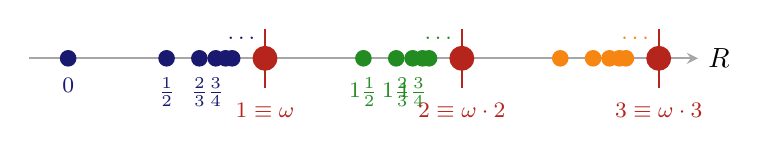
\begin{tikzpicture}[scale=2.5, >=stealth]
    % Axis
    \draw[->, thick, gray!70] (-0.2, 0) -- (3.2, 0) node[right, black] {$\mathbb{R}$};

    % Ticks and points for the first sequence (approaching 1)
    \foreach \n in {1, 2, 3, 4, 5, 6} {
        \pgfmathsetmacro{\x}{1 - 1/\n}
        \fill[MidnightBlue] (\x, 0) circle (1.2pt);
    }
    \node[below, MidnightBlue] at (0, -0.05) {\footnotesize $0$};
    \node[below, MidnightBlue] at (0.5, -0.05) {\footnotesize $\frac{1}{2}$};
    \node[below, MidnightBlue] at (0.667, -0.05) {\footnotesize $\frac{2}{3}$};
    \node[below, MidnightBlue] at (0.75, -0.05) {\footnotesize $\frac{3}{4}$};
    \node[MidnightBlue] at (0.88, 0.1) {\footnotesize $\dots$};

    % The limit point 1 (omega)
    \fill[BrickRed] (1, 0) circle (1.8pt);
    \draw[thick, BrickRed] (1, 0.15) -- (1, -0.15) node[below, yshift=-2pt] {\footnotesize $1 \equiv \omega$};

    % Ticks and points for the second sequence (approaching 2)
    \foreach \n in {2, 3, 4, 5, 6} { % Startet ab 2, um Überlappung mit 1 zu vermeiden
        \pgfmathsetmacro{\x}{2 - 1/\n}
        \fill[ForestGreen] (\x, 0) circle (1.2pt);
    }
    \node[below, ForestGreen] at (1.5, -0.05) {\footnotesize $1\frac{1}{2}$};
    \node[below, ForestGreen] at (1.667, -0.05) {\footnotesize $1\frac{2}{3}$};
    \node[below, ForestGreen] at (1.75, -0.05) {\footnotesize $1\frac{3}{4}$};
    \node[ForestGreen] at (1.88, 0.1) {\footnotesize $\dots$};

    % The limit point 2 (2*omega)
    \fill[BrickRed] (2, 0) circle (1.8pt);
    \draw[thick, BrickRed] (2, 0.15) -- (2, -0.15) node[below, yshift=-2pt] {\footnotesize $2 \equiv \omega \cdot 2$};

    % Ticks and points for the third sequence (approaching 3)
    \foreach \n in {2, 3, 4, 5, 6} { % Startet ab 2, um Überlappung mit 2 zu vermeiden
        \pgfmathsetmacro{\x}{3 - 1/\n}
        \fill[BurntOrange] (\x, 0) circle (1.2pt);
    }
    \node[BurntOrange] at (2.88, 0.1) {\footnotesize $\dots$};

    % The limit point 3 (3*omega)
    \fill[BrickRed] (3, 0) circle (1.8pt);
    \draw[thick, BrickRed] (3, 0.15) -- (3, -0.15) node[below, yshift=-2pt] {\footnotesize $3 \equiv \omega \cdot 3$};

\end{tikzpicture}
\end{center}
\end{math-stroke}

\begin{spoken-clean}[00:56:40 - 00:58:10]
Gut. Dann noch einmal zu der transfiniten Rekursion: Die Funktion $f$ besagt hier wirklich Folgendes: Wenn Sie eine Ordinalzahl $\beta < \lambda$ betrachten, dann haben Sie eine Folge von Elementen in $A$, die durch $\beta$ indiziert ist. Und die Funktion $f$ gibt Ihnen nun an, wie Sie aus dieser bisherigen Folge das nächste Folgenglied berechnen.

Das ist genau wie bei den Fibonacci-Zahlen, wo wir $F_n$ über die vorherigen Glieder als $F_{n-1} + F_{n-2}$ definiert haben.
\end{spoken-clean}

\begin{spoken-clean}[00:58:10 - 00:59:10]
Das heißt: Selbst ohne im Vorhinein die expliziten Werte aller vorherigen Glieder zu kennen, können wir --- basierend auf der gesamten bisherigen Folge bis hinunter zu $F_0$ --- das jeweils nächste Glied berechnen. Genau das ist die Aufgabe der Funktion $f$.

Wenn man diese Vorgabe hat, liefert uns das eine eindeutige transfinite Folge. Das ist die grundlegende Idee hinter der transfiniten Rekursion und Induktion, mit der man sehr viele mathematische Sätze beweisen kann.

Es gibt zwei berühmte Aussagen, die dieses Prinzip auf eine besonders nützliche Weise ausdrücken und ebenfalls zum Auswahlaxiom äquivalent sind. Das sind auch diejenigen Formulierungen, auf die man in der mathematischen Praxis am häufigsten stößt. Die erste davon ist das Kuratowski-Zorn-Lemma.
\end{spoken-clean}

\section{Äquivalenzen des Auswahlaxioms}
\subsection{Das Kuratowski-Zorn-Lemma}

\begin{spoken-clean}[00:59:10 - 01:00:26]
Das Kuratowski-Zorn-Lemma --- abgekürzt KZL. Lassen Sie sich nicht verwirren, wenn Sie diesem Satz in anderen mathematischen Büchern oder Papers begegnen: Mit hoher Wahrscheinlichkeit wird er dort einfach als \qt{Zorns Lemma} bezeichnet. Kuratowski verschwindet in der Standardliteratur meistens aus dem Namen.

Der Grund dafür ist historischer Natur. Lorenz Halbeisen interessiert sich sehr für die Geschichte der Mathematik und möchte Kuratowski die verdiente Anerkennung zukommen lassen, da dieser das Lemma tatsächlich etwa zehn Jahre vor Zorn formuliert hat. Es ist natürlich ein bisschen ungerecht, dass es heute fast nur nach Zorn benannt wird, aber die Namensgebung in der Mathematik ist selten gerecht. Nur weil ein Satz den Namen einer bestimmten Person trägt, bedeutet das keineswegs, dass diese Person ihn auch als Erste entdeckt hat. Daran muss man sich einfach gewöhnen --- Pech für Kuratowski, Glück für Zorn. Wir sind hier aber fair und nennen es das Kuratowski-Zorn-Lemma.

Ich frage mich übrigens manchmal, wie Mathematiker das sehen: Ich habe oft das Gefühl, das ultimative Ziel in der Mathematik ist es gar nicht, dass ein großer Satz nach einem benannt wird, sondern ein Lemma. Es gibt einige weltberühmte Hilfssätze, die jeder kennt --- wie das Lemma von Zorn oder das Lemma von Lax-Milgram. Warum eigentlich kein Hauptsatz? Wie dem auch sei: Wir bleiben höflich und nennen es das Kuratowski-Zorn-Lemma.
\end{spoken-clean}

\begin{spoken-clean}[01:00:26 - 01:00:45]
Wissen Sie noch, was das Kuratowski-Zorn-Lemma besagt? Das haben Sie ja bereits vorletzte Woche besprochen. Ja?
\end{spoken-clean}

\begin{student-interaction}[Studentenantwort]
Jede Kette hat eine obere Schranke\dots
\end{student-interaction}

\begin{spoken-clean}[01:00:45 - 01:01:39]
Genau, man muss bei der Formulierung ein bisschen präzise sein, aber das ist im Wesentlichen die Idee. Wenn wir eine nicht-leere, partiell geordnete Menge haben, in der jede Kette eine obere Schranke besitzt, dann hat diese Menge mindestens ein maximales Element.
\end{spoken-clean}

\begin{math-stroke}
\begin{theorem}[Kuratowski-Zorn-Lemma -- \emph{KZL}]\label[theorem]{thm:kuratowski-zorn-lemma-actual}
Sei $(P, \le)$ eine nicht-leere partiell geordnete Menge, sodass jede Kette $C \subseteq P$ eine obere Schranke in $P$ besitzt. Dann hat $P$ mindestens ein maximales Element.
\end{theorem}

\begin{explanation-of-steps}[Begrifflichkeiten der partiellen Ordnung]
Zur Erinnerung an die Definitionen aus der Ordnungstheorie:
\begin{itemize}
    \item \textbf{Partielle Ordnung:} Eine Relation $\le$ auf $P$, die reflexiv, antisymmetrisch und transitiv ist.
    \item \textbf{Kette:} Eine Teilmenge $C \subseteq P$, die bezüglich $\le$ total geordnet ist, d.\,h. für alle $x, y \in C$ gilt $x \le y$ oder $y \le x$.
    \item \textbf{Obere Schranke:} Ein Element $u \in P$, sodass $c \le u$ für alle $c \in C$ gilt.
    \item \textbf{Maximales Element:} Ein Element $m \in P$, sodass aus $m \le x$ für ein $x \in P$ stets $m = x$ folgt.
\end{itemize}
\end{explanation-of-steps}
\end{math-stroke}

\begin{spoken-clean}[01:01:39 - 01:04:13]
Man muss dieses Lemma ein paar Mal selbst angewendet haben, um zu sehen, warum es so unglaublich nützlich ist. Wir betrachten eine Menge, die nur partiell geordnet ist. Typischerweise ist das eine Familie von Teilmengen, die durch die Inklusion $\subseteq$ partiell geordnet ist. Das ist die klassische Anwendung: Sie haben eine Menge, dann eine größere Menge, aber das System ist nicht total geordnet, da zwei Mengen nicht zwingend ineinander enthalten sein müssen.

Die entscheidende Bedingung ist nun: Wenn Sie eine Kette haben --- also eine Familie von Elementen, die bezüglich der Ordnung immer größer werden ---, dann muss es ein Element in $P$ geben, das eine obere Schranke für diese Kette bildet. Wenn das für jede Kette erfüllt ist, dann garantiert das Lemma, dass $P$ ein maximales Element besitzt.

Sie haben diese Begriffe vorletzte Woche sicherlich alle im Detail definiert. Auf dem aktuellen Übungsblatt sollen Sie nun mithilfe des Kuratowski-Zorn-Lemmas beweisen, dass jeder Vektorraum eine Basis besitzt. Sie werden sehen, dass die Anwendung dieses Lemmas oft viel eleganter und einfacher ist, als den Beweis über die transfinite Rekursion zu führen.
\end{spoken-clean}

\begin{didactic-insight}[Die intuitive Funktionsweise von KZL]
Das Kuratowski-Zorn-Lemma ist ein extrem mächtiges Werkzeug in der unendlichen Dimension. Es erlaubt uns, die Existenz von maximalen Objekten (wie Basen in Vektorräumen, maximalen Idealen in Ringen oder Wohlordnungen auf Mengen) zu beweisen, ohne diese explizit konstruieren zu müssen. Die Bedingung, dass jede Kette eine obere Schranke besitzt, sichert ab, dass wir beim sukzessiven \qt{Vergrößern} unserer Objekte nicht in eine Sackgasse geraten, sondern die Kette durch ihre Vereinigung nach oben beschränken können.
\begin{align*}
  \text{Kette } C_0 \subseteq C_1 \subseteq C_2 \subseteq \dots \implies \bigcup_{i} C_i \in P \quad \text{(obere Schranke)}
\end{align*}
\end{didactic-insight}

\begin{spoken-clean}[01:04:13 - 01:06:34]
In der mathematischen Praxis nutzt man das Lemma sehr häufig, um die Existenz einer Basis in beliebigen Vektorräumen zu beweisen. Die Intuition dahinter ist genau dieselbe wie bei unserer transfiniten Konstruktion: Sie betrachten die Familie aller linear unabhängigen Teilmengen des Vektorraums. Wenn Sie eine Kette solcher Mengen haben, liefert die Vereinigung aller Elemente dieser Kette wieder eine linear unabhängige Teilmenge und somit eine obere Schranke.

Mit dem Kuratowski-Zorn-Lemma folgt dann sofort, dass ein maximales Element existieren muss --- und eine maximale linear unabhängige Teilmenge ist genau eine Basis. Das ist die ganze Idee: Man nimmt eine Menge linear unabhängiger Vektoren und fügt so lange weitere Vektoren hinzu, bis es nicht mehr weitergeht. Dann hat man eine Basis.

Das klingt anschaulich völlig harmlos und natürlich. Da unsere unendlichen Mengen aber beliebig groß sein können, müssen wir diesen Prozess formal absolut präzise absichern --- und genau dafür benötigen wir solche mächtigen Sätze. Als Nächstes gibt es noch das Teichmüller-Prinzip.
\end{spoken-clean}

\subsection{Das Teichmüller-Prinzip}

\begin{spoken-clean}[01:06:34 - 01:08:33]
Oswald Teichmüller war ein herausragender Mathematiker in den 1930er-Jahren in Deutschland, charakterlich allerdings eine sehr problematische Figur: Er war ein überzeugter Nationalsozialist, meldete sich freiwillig für den Kriegsdienst an der Ostfront und fiel dort auch. Dennoch hat er viele mathematisch sehr einflussreiche Resultate bewiesen.

Das Teichmüller-Prinzip besagt: Wenn $\mathcal{F}$ eine nicht-leere Familie von Mengen mit endlichem Charakter ist, dann besitzt $\mathcal{F}$ ein bezüglich der Inklusion maximales Element. Auch hier sieht man sofort, wie gut das für Vektorräume funktioniert: Die Eigenschaft einer Teilmenge, linear unabhängig zu sein, hat endlichen Charakter. Mit dem Teichmüller-Prinzip folgt daraus direkt die Existenz einer maximalen linear unabhängigen Teilmenge, was, wie wir wissen, genau eine Basis des Vektorraums ist.
\end{spoken-clean}

\begin{math-stroke}
\begin{definition}[Endlicher Charakter]\label[definition]{def:endlicher-charakter-actual}
Eine Familie $\mathcal{F}$ von Mengen hat \newterm{endlichen Charakter}, falls für jede Menge $X$ gilt:
\begin{equation}\label{eq:endlicher-charakter-actual}
X \in \mathcal{F} \iff \text{Jede endliche Teilmenge } E \subseteq X \text{ liegt in } \mathcal{F}.
\end{equation}
\end{definition}

\begin{theorem}[Teichmüller-Prinzip -- \emph{TP}]\label[theorem]{thm:teichmueller-prinzip-actual}
Jede nicht-leere Familie $\mathcal{F}$ von Mengen mit endlichem Charakter besitzt ein bezüglich Inklusion ($\subseteq$) maximales Element.
\end{theorem}

\begin{explanation-of-steps}[Anwendung auf die lineare Unabhängigkeit]
Die Eigenschaft der linearen Unabhängigkeit in einem Vektorraum $V$ hat endlichen Charakter:
Eine beliebige Teilmenge $X \subseteq V$ ist genau dann linear unabhängig, wenn jede endliche Teilmenge $E \subseteq X$ linear unabhängig ist. Das Teichmüller-Prinzip liefert daher sofort die Existenz einer maximalen linear unabhängigen Teilmenge, welche eine Basis von $V$ bildet.
\end{explanation-of-steps}
\end{math-stroke}

\begin{spoken-clean}[01:08:33 - 01:10:28]
Was wir jetzt beweisen wollen, ist der folgende Äquivalenzsatz. Er besagt, dass die folgenden Aussagen alle zum Auswahlaxiom äquivalent sind: Erstens das Wohlordnungsprinzip --- das haben Sie bereits gesehen ---, zweitens das Kuratowski-Zorn-Lemma und drittens das Teichmüller-Prinzip.

Ich habe in den Vorlesungsnotizen von Fabian Ziltener ein amüsantes Zitat dazu gefunden. Er schreibt sinngemäß: Beim Auswahlaxiom ist völlig offensichtlich, dass es wahr sein muss; beim Wohlordnungsprinzip ist völlig offensichtlich, dass es falsch sein muss; und beim Lemma von Zorn oder dem Teichmüller-Prinzip ist es schlicht unklar, ob sie offensichtlich sind oder nicht.

Aber genau das ist das Faszinierende am Auswahlaxiom: Es verbindet Aussagen, die intuitiv völlig einleuchtend wirken, mit solchen, die auf den ersten Blick völlig kontraintuitiv erscheinen.
\end{spoken-clean}

\begin{math-stroke}
\begin{theorem}[Äquivalente Formulierungen von \emph{AC}]\label[theorem]{thm:ac-equivalenzen-actual}
In der Zermelo-Fraenkel-Mengenlehre (\emph{ZF}) sind die folgenden Aussagen äquivalent:
\begin{enumerate}[label=\textbf{(\arabic*)}]
    \item \textbf{Auswahlaxiom} (\emph{AC})
    \item \textbf{Wohlordnungsprinzip} (\emph{WOP})
    \item \textbf{Kuratowski-Zorn-Lemma} (\emph{KZL})
    \item \textbf{Teichmüller-Prinzip} (\emph{TP})
\end{enumerate}
\end{theorem}
\end{math-stroke}

\subsection{Beweis des Äquivalenzsatzes}

\begin{spoken-clean}[01:10:28 - 01:13:04]
Kommen wir zum Beweis. Wir haben bereits gesehen, dass das Auswahlaxiom und das Wohlordnungsprinzip äquivalent sind (i.e., $\text{AC} \iff \text{WOP}$). Nun wollen wir zeigen, dass das Wohlordnungsprinzip das Kuratowski-Zorn-Lemma impliziert (i.e., $\text{WOP} \implies \text{KZL}$).

Wir führen den Beweis über einen Ringschluss: von WOP zu KZL, von KZL zu TP, und von TP zurück zu AC. Für den ersten Schritt nutzen wir wieder die transfinite Rekursion. Sei $(P, \le)$ eine nicht-leere partielle Ordnung. Nach dem Wohlordnungsprinzip können wir die Elemente von $P$ durch die Elemente einer Ordinalzahl $\lambda \in \Omega$ indizieren, das heißt: $P = \{p_\beta \mid \beta \in \lambda\}$.
\end{spoken-clean}

\begin{proof}[Beweis des Äquivalenzsatzes]
Wir führen den Beweis über den Zyklus $\text{WOP} \implies \text{KZL} \implies \text{TP} \implies \text{AC}$.

\begin{math-stroke}[Teil 1: WOP $\implies$ KZL]
Sei $(P, \le)$ eine nicht-leere partiell geordnete Menge, in der jede Kette eine obere Schranke besitzt. 

Nach dem Wohlordnungsprinzip (\emph{WOP}) existiert eine Wohlordnung auf $P$. Wir können die Elemente von $P$ daher durch eine Ordinalzahl $\lambda \in \Omega$ indizieren:
\[
P = \{p_\beta \mid \beta \in \lambda\}.
\]
\end{math-stroke}

\subsection{Definition der Rekursionsfunktion für KZL}
\begin{spoken-clean}[01:13:04 - 01:15:50]
Nun wollen wir eine passende Rekursionsfunktion $f$ definieren. Wie üblich beginnen wir für $\beta = 0$ mit der leeren Menge: Wir setzen $f(t) = \emptyset$, falls $\beta = 0$ ist.

Um den Schritt von $\delta$ zu $\delta+1$ zu machen, gehen wir wie folgt vor: Wenn die bisher konstruierte Menge $t(\delta)$ eine Kette ist und das neue Element $p_\delta$ eine obere Schranke für diese Kette darstellt, dann fügen wir es hinzu. Andernfalls tun wir nichts. Auf diese Weise konstruieren wir eine aufsteigende Kette. Unsere Funktion $f(t)$ sieht also wie folgt aus\dots
\end{spoken-clean}

\begin{spoken-clean}[01:15:50 - 01:18:35]
Wir definieren $f(t)$ im Rekursionsschritt wie folgt: Es ist die leere Menge $\emptyset$, falls $\beta = 0$ ist.

Für den Nachfolgerschritt $\beta = \delta + 1$ setzen wir $f(t) = t(\delta)$, falls $t(\delta)$ keine Kette ist --- dieser Fall dient nur der formalen Vollständigkeit und tritt in der Konstruktion eigentlich gar nicht auf. Ebenfalls $t(\delta)$ setzen wir, falls $t(\delta)$ zwar eine Kette ist, aber $p_\delta$ keine obere Schranke für $t(\delta)$ darstellt. In diesem Fall verändern wir die Menge also nicht.

Wenn $p_\delta$ jedoch eine obere Schranke für die Kette $t(\delta)$ ist --- das heißt, es ist mit allen Elementen in $t(\delta)$ vergleichbar und größer oder gleich diesen ---, dann fügen wir es hinzu: Wir setzen $f(t) = t(\delta) \cup \{p_\delta\}$, falls $t(\delta)$ eine Kette und $p_\delta$ eine obere Schranke für $t(\delta)$ ist.

Und schließlich für den Fall, dass $\beta$ eine Limes-Ordinalzahl ist, nehmen wir einfach die Vereinigung aller bisherigen Glieder, also die Vereinigung über alle $\gamma < \beta$.
\end{spoken-clean}

\begin{math-stroke}[Definition der Rekursionsfunktion für KZL]
Wir definieren die Rekursionsfunktion $f \colon \bigcup_{\beta < \lambda} {}^{\displaystyle \beta}\!\mathcal{P}(P) \to \mathcal{P}(P)$ für eine Funktion $t \colon \beta \to \mathcal{P}(P)$ durch:
\begin{equation}\label{eq:kzl-rekursion-f-actual}
f(t) := \begin{cases}
\emptyset & \text{falls } \beta = 0, \\[1.3em]
t(\delta) & \parbox{0.54\textwidth}{\raggedright falls $\beta = \delta + 1$ und $t(\delta)$ ist keine Kette,} \\[1.3em]
t(\delta) & \parbox{0.54\textwidth}{\raggedright falls $\beta = \delta + 1$ und $t(\delta)$ ist Kette, aber $p_\delta$ ist keine obere Schranke für $t(\delta)$,} \\[1.3em]
t(\delta) \cup \{p_\delta\} & \parbox{0.54\textwidth}{\raggedright falls $\beta = \delta + 1$ und $t(\delta)$ ist Kette, und $p_\delta$ ist eine obere Schranke für $t(\delta)$,} \\[1.3em]
\displaystyle\bigcup_{\gamma < \beta} t(\gamma) & \text{falls } \beta \text{ eine Limes-Ordinalzahl ist}.
\end{cases}
\end{equation}
\end{math-stroke}

\subsection{Konstruktion der Kette}
\begin{spoken-clean}[01:18:35 - 01:21:38]
Soweit zur Rekursionsdefinition. Wir fügen das jeweils nächste Element also genau dann hinzu, wenn es harmonisch in die Kette passt. Wir beginnen bei $0$, fügen ein Element hinzu, und wenn das nächste Element größer ist als die bisherigen, nehmen wir es auf; ist es nicht vergleichbar, lassen wir es weg. So erhalten wir eine wohldefinierte Kette.

Nach dem Satz über die transfinite Rekursion existiert nun eine eindeutige Funktion $a$ von $\lambda$ in die Potenzmenge $\mathcal{P}(P)$, sodass $a(\beta) = f(a|_{\beta})$ für alle $\beta \in \lambda$ gilt. Wir definieren wieder $A_\beta := a(\beta)$ und setzen $B := \bigcup_{\beta \in \lambda} A_\beta$ als die Vereinigung all dieser Mengen. Die Behauptung ist nun, dass diese Menge $B$ eine Kette in $P$ ist.
\end{spoken-clean}

\begin{math-stroke}[Konstruktion der Kette]
Nach dem Satz über die transfinite Rekursion (\cref{thm:transfinite-rekursion-existenz}) existiert eine eindeutige Funktion $a \colon \lambda \to \mathcal{P}(P)$, sodass für alle $\beta \in \lambda$ gilt:
\[
a(\beta) = f(a|_{\beta}).
\]
Wir definieren für jedes $\beta \in \lambda$ die Teilmenge $A_\beta := a(\beta) \subseteq P$. 
Die Vereinigung aller Glieder dieser rekursiven Kette ist:
\begin{equation}\label{eq:kzl-kette-vereinigung-actual}
B := \bigcup_{\beta \in \lambda} A_\beta.
\end{equation}
\begin{claim}\label[claim]{clm:kzl-kette-actual}
Die Menge $B$ ist eine Kette in $P$.
\end{claim}
\begin{short-proof}[Beweis der Ketteneigenschaft]
Dies folgt direkt per transfiniter Induktion über die Konstruktion von $f(t)$ in \eqref{eq:kzl-rekursion-f-actual}, da in jedem Nachfolgerschritt ein Element $p_\delta$ nur dann hinzugefügt wird, wenn es eine obere Schranke für die bisherige Kette $t(\delta)$ darstellt.
\end{short-proof}
\end{math-stroke}

\subsection{Nachweis der Maximalität}
\begin{spoken-clean}[01:21:38 - 01:24:00]
Die zweite Behauptung ist nun, dass jede obere Schranke $m$ von $B$ ein maximales Element in $P$ sein muss. Das folgt im Wesentlichen direkt aus unserer Konstruktion: Angenommen, diese obere Schranke $m$ wäre nicht maximal. Dann müsste ein Element $p_\delta \in P$ existieren mit $m < p_\delta$.

Daraus folgt jedoch, dass $p_\delta$ auch eine obere Schranke für $A_\delta$ sein muss, da $A_\delta \subseteq B$ per Definition gilt. Nach unserer Rekursionsdefinition von $f$ müssten wir beim Schritt zu $A_{\delta+1}$ das Element $p_\delta$ hinzufügen, sodass $p_\delta \in A_{\delta+1} \subseteq B$ gelten würde. Da $m$ aber eine obere Schranke von $B$ ist, müsste $p_\delta \le m$ gelten --- was im direkten Widerspruch zu unserer Annahme $m < p_\delta$ steht.

Dieser Widerspruch zeigt, dass die obere Schranke $m$ tatsächlich ein maximales Element von $P$ sein muss. Damit ist bewiesen, dass ein maximales Element existiert.
\end{spoken-clean}

\begin{math-stroke}[Nachweis der Maximalität]
\begin{claim}\label[claim]{clm:kzl-maximales-element-actual}
Die Kette $B$ besitzt eine obere Schranke $m \in P$, welche ein maximales Element von $P$ ist.
\end{claim}
\begin{short-proof}[Beweis der Maximalität]
Nach Voraussetzung des Lemmas besitzt die Kette $B$ eine obere Schranke $m \in P$. Angenommen, $m$ ist nicht maximal. Dann existiert ein Element $p_\delta \in P$ mit $m < p_\delta$. 

Da $m$ eine obere Schranke von $B$ ist, ist $p_\delta$ ebenfalls eine obere Schranke für alle $A_\gamma$ mit $\gamma \le \delta$. Nach Konstruktion der Rekursionsfunktion $f$ in \eqref{eq:kzl-rekursion-f-actual} gilt für den Schritt $\beta = \delta + 1$:
\[
A_{\delta+1} = A_\delta \cup \{p_\delta\}.
\]
Daraus folgt $p_\delta \in A_{\delta+1} \subseteq B$. Da $m$ eine obere Schranke von $B$ ist, muss $p_\delta \le m$ gelten. Dies steht im direkten Widerspruch zu unserer Annahme $m < p_\delta$. 

Daraus schließen wir, dass die obere Schranke $m$ ein maximales Element der Menge $P$ ist. Damit ist die Implikation $\text{WOP} \implies \text{KZL}$ bewiesen.
\end{short-proof}
\end{math-stroke}

\subsection{Teil 2: KZL \texorpdfstring{$\implies$}{implies} TP}
\begin{spoken-clean}[01:24:00 - 01:26:34]
Somit haben wir gezeigt, dass aus dem Wohlordnungsprinzip das Kuratowski-Zorn-Lemma folgt. Als Nächstes beweisen wir, dass das Kuratowski-Zorn-Lemma das Teichmüller-Prinzip impliziert (i.e., $\text{KZL} \implies \text{TP}$).

Sei $\mathcal{F}$ eine nicht-leere Familie von Mengen mit endlichem Charakter. Wir wollen zeigen, dass das Teichmüller-Prinzip gilt. Dazu betrachten wir die partielle Ordnung $(\mathcal{F}, \subseteq)$. Um das Kuratowski-Zorn-Lemma anzuwenden, müssen wir zeigen, dass jede Kette $\mathcal{C} \subseteq \mathcal{F}$ eine obere Schranke in $\mathcal{F}$ besitzt. Wir definieren diese obere Schranke als die Vereinigung $U := \bigcup \mathcal{C}$.

Ich skizziere die Beweisidee kurz zu Ende, wenn ich darf: Da $\mathcal{F}$ endlichen Charakter besitzt, können wir zeigen, dass diese Vereinigung $U$ ebenfalls in $\mathcal{F}$ liegt, indem wir nachweisen, dass jede endliche Teilmenge von $U$ in $\mathcal{F}$ liegt. Da $\mathcal{C}$ eine Kette ist, ist jede endliche Teilmenge von $U$ in einem Element der Kette enthalten, welches in $\mathcal{F}$ liegt. Somit ist $U \in \mathcal{F}$ eine obere Schranke. Nach dem Kuratowski-Zorn-Lemma existiert folglich ein maximales Element in $\mathcal{F}$. Das ist die Beweisidee in aller Kürze. Die vollständigen Details finden Sie im Skript von Lorenz Halbeisen --- Sie können sich das gerne in Ruhe anschauen, selbst durchdenken oder in den Übungsstunden mit den Assistenten diskutieren.
\end{spoken-clean}

\begin{math-stroke}[Teil 2: KZL $\implies$ TP]
\begin{short-proof}[Beweis von KZL $\implies$ TP]
Sei $\mathcal{F}$ eine nicht-leere Familie von Mengen mit endlichem Charakter. Wir betrachten die partiell geordnete Menge $(\mathcal{F}, \subseteq)$. 

Um das Kuratowski-Zorn-Lemma anzuwenden, müssen wir zeigen, dass jede Kette $\mathcal{C} \subseteq \mathcal{F}$ eine obere Schranke in $\mathcal{F}$ besitzt. Wir definieren den Kandidaten für die obere Schranke als die Vereinigung der Kette:
\[
U := \bigcup \mathcal{C} = \bigcup_{X \in \mathcal{C}} X.
\]
Wir zeigen nun, dass $U \in \mathcal{F}$ gilt. Da $\mathcal{F}$ endlichen Charakter hat, reicht es nach Definition \ref{def:endlicher-charakter-actual} zu zeigen, dass jede endliche Teilmenge $E \subseteq U$ in $\mathcal{F}$ liegt:
\begin{itemize}
    \item Sei $E = \{x_1, \dots, x_k\} \subseteq U$ eine beliebige endliche Teilmenge.
    \item Für jedes $x_i \in E$ existiert ein Element $X_i \in \mathcal{C}$ mit $x_i \in X_i$.
    \item Da $\mathcal{C}$ eine Kette ist, ist die endliche Teilmenge $\{X_1, \dots, X_k\} \subseteq \mathcal{C}$ bezüglich Inklusion total geordnet. Es existiert somit ein maximales Element $X_{\max} \in \{X_1, \dots, X_k\}$, sodass $X_i \subseteq X_{\max}$ für alle $i \in \{1, \dots, k\}$ gilt.
    \item Daraus folgt unmittelbar $E \subseteq X_{\max}$.
    \item Da $X_{\max} \in \mathcal{C} \subseteq \mathcal{F}$ und $\mathcal{F}$ endlichen Charakter hat, muss auch die Teilmenge $E \in \mathcal{F}$ sein.
\end{itemize}
Da jede endliche Teilmenge $E \subseteq U$ in $\mathcal{F}$ liegt, folgt $U \in \mathcal{F}$. Somit ist $U$ eine obere Schranke für die Kette $\mathcal{C}$ in $\mathcal{F}$.

Nach dem Kuratowski-Zorn-Lemma (\cref{thm:kuratowski-zorn-lemma-actual}) besitzt $(\mathcal{F}, \subseteq)$ ein maximales Element. Dies beweist $\text{KZL} \implies \text{TP}$.
\end{short-proof}
\end{math-stroke}

\subsection{Teil 3: TP \texorpdfstring{$\implies$}{implies} AC}
\begin{spoken-clean}[01:26:34 - 01:28:40]
Gut. Jetzt beweisen wir noch den letzten Schritt: dass das Teichmüller-Prinzip das Auswahlaxiom impliziert (i.e., $\text{TP} \implies \text{AC}$).

Wenn wir eine Familie $\mathcal{F}$ von nicht-leeren Mengen haben, wollen wir eine Auswahlfunktion konstruieren. Dazu definieren wir uns ein System $\mathcal{S}$ von partiellen Auswahlfunktionen. Wir betrachten die Menge aller Funktionen $g$, deren Definitionsbereich eine Teilfamilie $\mathcal{F}' \subseteq \mathcal{F}$ ist, sodass $g(X) \in X$ für alle $X \in \mathcal{F}'$ gilt. Wir können diese Funktionen formal als Mengen von geordneten Paaren interpretieren.
\end{spoken-clean}

\begin{math-stroke}[Teil 3: TP $\implies$ AC]
\begin{short-proof}[Beweis von TP $\implies$ AC]
Sei $\mathcal{F}$ eine Familie von nicht-leeren Mengen. Wir wollen die Existenz einer Auswahlfunktion $f \colon \mathcal{F} \to \bigcup \mathcal{F}$ zeigen.

Wir definieren die Familie $\mathcal{S}$ aller partiellen Auswahlfunktionen auf $\mathcal{F}$:
\begin{equation}\label{eq:partielle-auswahlfunktionen-actual}
\begin{split}
\mathcal{S} := \Biggl\{ g \subseteq \mathcal{F} \times \bigcup \mathcal{F} \;\Biggm|\; & g \text{ ist eine Funktion, } \operatorname{dom}(g) \subseteq \mathcal{F} \\
& \text{und } \forall X \in \operatorname{dom}(g) \, (g(X) \in X) \Biggr\}.
\end{split}
\end{equation}
Wir zeigen, dass die Familie $\mathcal{S}$ endlichen Charakter besitzt:
\begin{itemize}
    \item Eine Relation $g$ ist genau dann eine Funktion in $\mathcal{S}$, wenn jede endliche Teilmenge von Paaren in $g$ eine eindeutige Zuordnung definiert und die Auswahlbedingung erfüllt. Dies ist eine rein lokale Eigenschaft, die sich auf endliche Teilmengen reduzieren lässt. \inlinemetanote{[Anmerkung: ($\Rightarrow$) Jede Teilmenge einer partiellen Auswahlfunktion ist wieder eine. ($\Leftarrow$) Ist jede endliche Teilmenge von $g$ eine partielle Auswahlfunktion, so ist $g$ rechtseindeutig -- andernfalls gäbe es $y_1 \neq y_2$ mit $\langle x,y_1\rangle, \langle x,y_2\rangle \in g$, was in einer endlichen Teilmenge läge -- und es gilt $x \in X$ für alle $\langle X,x\rangle \in g$.]}
\end{itemize}
Da $\mathcal{S}$ nicht-leer ist ($\emptyset \in \mathcal{S}$) und endlichen Charakter besitzt, existiert nach dem Teichmüller-Prinzip (\cref{thm:teichmueller-prinzip-actual}) ein bezüglich Inklusion maximales Element $f_0 \in \mathcal{S}$.

Wir zeigen nun per Widerspruch, dass der Definitionsbereich von $f_0$ die gesamte Familie $\mathcal{F}$ sein muss (d.\,h. $\operatorname{dom}(f_0) = \mathcal{F}$):
\begin{itemize}
    \item Angenommen, $\operatorname{dom}(f_0) \neq \mathcal{F}$. Dann existiert eine Menge $Y \in \mathcal{F} \setminus \operatorname{dom}(f_0)$.
    \item Da $Y \in \mathcal{F}$, ist $Y$ nach Voraussetzung nicht-leer. Wir können somit ein Element $y \in Y$ wählen.
    \item Wir definieren die erweiterte Funktion $f'_0 := f_0 \cup \{(Y, y)\}$.
    \item Offensichtlich gilt $f_0 \subsetneq f'_0$ und $f'_0 \in \mathcal{S}$. Dies steht im direkten Widerspruch zur Maximalität von $f_0$ in $\mathcal{S}$.
\end{itemize}
Folglich gilt $\operatorname{dom}(f_0) = \mathcal{F}$. Die maximale partielle Auswahlfunktion $f_0$ ist somit eine vollständige Auswahlfunktion für $\mathcal{F}$. Dies beweist $\text{TP} \implies \text{AC}$ und schließt den Äquivalenzkreis.
\end{short-proof}
\end{math-stroke}

\begin{didactic-insight}[Einzelelement-Auswahl ohne AC]
Beachten Sie hier ein feines formallogisches Detail: Im Beweis sagen wir: \qt{Wir können somit ein Element $y \in Y$ wählen.} Um ein Element aus einer \emph{einzelnen} nicht-leeren Menge $Y$ zu wählen, benötigen wir das Auswahlaxiom \emph{nicht}. Die Existenz eines solchen Elements wird bereits durch die logische Schlussregel der Existenzbeseitigung (Existential Instantiation) in Verbindung mit der Prämisse $Y \neq \emptyset$ gesichert. Das Auswahlaxiom wird nur zwingend erforderlich, wenn wir \emph{simultan} für unendlich viele Mengen eine Auswahl treffen müssen, ohne eine explizite Konstruktionsregel angeben zu können.
\end{didactic-insight}
\end{proof}

\begin{spoken-clean}[01:28:40 - 01:29:21]
Gut, das schließt den Beweis für heute. Die Details zu diesen Äquivalenzen und den historischen Kontext finden Sie wie gewohnt im Skript von Lorenz Halbeisen. Sie können sich das gerne nochmals in Ruhe anschauen und in den Übungsstunden mit den Assistenten diskutieren.

Das Auswahlaxiom und seine Äquivalenzen sind ein faszinierendes Fundament, das uns zeigt, wie eng formale Logik und mathematische Intuition miteinander verflochten sind. Nächste Woche werden wir darauf aufbauen und uns den Kardinalzahlen widmen.

Ich bedanke mich ganz herzlich fürs Kommen, wünsche Ihnen eine erfolgreiche und erholsame Woche und wir sehen uns am nächsten Dienstag wieder hier im Hörsaal. Tschüss zusammen!
\end{spoken-clean}

\begin{nice-box}[Zusammenfassung der Schlüsselkonzepte]
In dieser Vorlesung haben wir die folgenden zentralen Konzepte und Resultate erarbeitet:
\begin{itemize}
    \item \textbf{Auswahlaxiom (AC):} Garantiert die Existenz einer Auswahlfunktion für jede Familie nicht-leerer Mengen. Es ist äquivalent dazu, dass das kartesische Produkt nicht-leerer Mengen nicht leer ist.
    \item \textbf{Ordinalzahlen:} Verallgemeinerung der natürlichen Zahlen für das transfinite Zählen. Sie sind transitive Mengen, die durch die Elementrelation $\in$ wohlgeordnet sind. Jede Ordinalzahl ist entweder $0$, eine Nachfolger-Ordinalzahl ($\beta + 1$) oder eine Limes-Ordinalzahl ($\bigcup \alpha$).
    \item \textbf{Transfinite Induktion \& Rekursion:} Mächtige Beweis- und Konstruktionsprinzipien über Ordinalzahlen. Die transfinite Rekursion ermöglicht beispielsweise den Beweis, dass jeder Vektorraum eine Basis besitzt.
    \item \textbf{Kuratowski-Zorn-Lemma (KZL):} Besagt, dass jede nicht-leere partiell geordnete Menge, in der jede Kette eine obere Schranke hat, mindestens ein maximales Element besitzt. Es ist ein unverzichtbares Werkzeug in der unendlichdimensionalen Algebra und Analysis.
    \item \textbf{Teichmüller-Prinzip (TP):} Garantiert ein maximales Element für jede nicht-leere Familie von Mengen mit endlichem Charakter.
    \item \textbf{Äquivalenzsatz:} Im Rahmen von ZF sind das Auswahlaxiom (AC), das Wohlordnungsprinzip (WOP), das Kuratowski-Zorn-Lemma (KZL) und das Teichmüller-Prinzip (TP) alle mathematisch äquivalent zueinander.
\end{itemize}
\end{nice-box}

% [SYSTEM] Refinement complete